% ==============================================================
% Section: Recursive Structure with Markov Risk
% ==============================================================

\section{Recursive Structure with Markov Risk}
\label{sec:recursive-markov}

In Chapter 5, we studied discounted sums and risk as weighted averages, treating shocks as independent over time. The recursive decomposition allowed us to express long (or infinite) horizon objects through simple one-step-ahead relationships. This section shows that the same recursive logic extends naturally to Markov risk---the key difference is that the weights in our generalized means now depend on the current state.

% --------------------------------------------------------------
\subsection{From Sequences to Trees}
\label{subsec:sequences-to-trees}
% --------------------------------------------------------------

Under i.i.d.\ uncertainty, a stochastic payoff stream can be visualized as a sequence: each period, nature draws from the same distribution, and the agent receives a payoff. The structure is ``flat'' in the sense that the probabilities governing tomorrow's outcome are the same regardless of today's realization.

With Markov uncertainty, the picture changes. From each state, the system branches into possible future states with state-dependent probabilities. The result is a \emph{tree} rather than a sequence: each node represents a state, and the branches represent transitions weighted by $\pi_{ij}$.

\paragraph{The Branch Tree.}
Consider a two-period example starting from state $i$. The agent receives $d(i)$ today. Tomorrow, the state transitions to $j$ with probability $\pi_{ij}$, yielding $d(j)$. The tree looks like:

\begin{center}
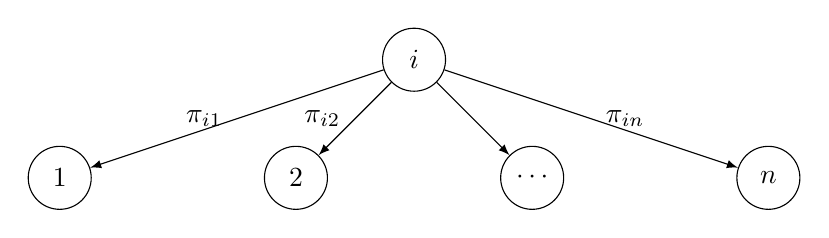
\begin{tikzpicture}[
    level 1/.style={sibling distance=30mm},
    level 2/.style={sibling distance=15mm},
    every node/.style={circle, draw, minimum size=8mm},
    edge from parent/.style={draw, -latex}
]
\node {$i$}
    child {node {$1$} edge from parent node[left, draw=none] {$\pi_{i1}$}}
    child {node {$2$} edge from parent node[left, draw=none] {$\pi_{i2}$}}
    child {node {$\cdots$} edge from parent node[right, draw=none] {}}
    child {node {$n$} edge from parent node[right, draw=none] {$\pi_{in}$}};
\end{tikzpicture}
\end{center}

The key insight is that this branching structure \emph{repeats} at each node: from state $j$, the system branches again according to row $j$ of the transition matrix. This self-similar structure is what makes recursion possible.

\begin{calloutimportant}[From Flat to Branching]
Under i.i.d.\ risk, the probability weights $\pi_s$ are constants---the same at every node. Under Markov risk, the weights $\pi_{ij}$ depend on the current node $i$. The recursive formulas from Chapter 5 carry over, but with state-dependent weights replacing fixed weights.
\end{calloutimportant}

% --------------------------------------------------------------
\subsection{Present Value with Markov Risk}
\label{subsec:present-value-markov}
% --------------------------------------------------------------

Consider a payoff stream $\{d(s_t)\}$ where the payoff depends on the current state. What is the present value of this stream, starting from state $i$?

\paragraph{The Recursive Formula.}
Let $V(i)$ denote the present value starting from state $i$. The agent receives $d(i)$ today and, from tomorrow onward, receives the present value $V(j)$ with probability $\pi_{ij}$. Discounting at rate $\beta$:
\begin{equation}
V(i) = d(i) + \beta \sum_{j=1}^{n} \pi_{ij} V(j).
\label{eq:pv-recursive}
\end{equation}
This is a system of $n$ linear equations, one for each state.

\paragraph{Matrix Notation.}
Let $\mathbf{V} = (V(1), \ldots, V(n))^\top$ and $\mathbf{d} = (d(1), \ldots, d(n))^\top$ be column vectors. Then \eqref{eq:pv-recursive} becomes:
\begin{equation}
\mathbf{V} = \mathbf{d} + \beta \Pi \mathbf{V}.
\label{eq:pv-matrix}
\end{equation}
This is precisely the fixed-point equation from Chapter 5, now with $\Pi$ replacing the scalar discount factor.

\paragraph{The Inversion Formula.}
Rearranging \eqref{eq:pv-matrix}:
\begin{equation}
(I - \beta \Pi) \mathbf{V} = \mathbf{d},
\label{eq:pv-rearranged}
\end{equation}
which yields the closed-form solution:
\begin{equation}
\boxed{\mathbf{V} = (I - \beta \Pi)^{-1} \mathbf{d}.}
\label{eq:pv-inversion}
\end{equation}

The matrix $(I - \beta \Pi)^{-1}$ is the \emph{resolvent} of the discounted transition operator. It exists whenever $\beta < 1$ (or more generally, whenever $\beta$ times the spectral radius of $\Pi$ is less than one---which holds since $\Pi$ is stochastic and has spectral radius 1).

\begin{calloutnote}[Geometric Series Interpretation]
The resolvent has a power series expansion:
\begin{equation}
(I - \beta \Pi)^{-1} = I + \beta \Pi + \beta^2 \Pi^2 + \beta^3 \Pi^3 + \cdots = \sum_{t=0}^{\infty} \beta^t \Pi^t.
\label{eq:resolvent-series}
\end{equation}
The $(i,j)$ entry of $\beta^t \Pi^t$ is the discounted probability of being in state $j$ after $t$ periods, starting from state $i$. The present value sums these discounted probabilities times payoffs across all future dates and states.
\end{calloutnote}

\paragraph{Example: Two-State Present Value.}
For the boom-recession chain with $\mathbf{d} = (d_B, d_R)^\top$ (payoffs in boom and recession):
\begin{equation}
I - \beta \Pi = \begin{pmatrix}
1 - 0.9\beta & -0.1\beta \\
-0.3\beta & 1 - 0.7\beta
\end{pmatrix}.
\label{eq:two-state-resolvent-matrix}
\end{equation}
Inverting (with determinant $\Delta = (1-0.9\beta)(1-0.7\beta) - 0.03\beta^2$):
\begin{equation}
\mathbf{V} = \frac{1}{\Delta} \begin{pmatrix}
1 - 0.7\beta & 0.1\beta \\
0.3\beta & 1 - 0.9\beta
\end{pmatrix} \begin{pmatrix} d_B \\ d_R \end{pmatrix}.
\label{eq:two-state-pv}
\end{equation}
The present value in booms exceeds that in recessions when $d_B > d_R$ and booms are persistent.

% --------------------------------------------------------------
\subsection{Certainty Equivalents with State-Dependent Probabilities}
\label{subsec:ce-markov}
% --------------------------------------------------------------

We now connect Markov risk to the generalized mean framework from Chapter 5. The certainty equivalent becomes state-dependent, with each state using its own row of the transition matrix as probability weights.

\paragraph{State-Contingent Certainty Equivalent.}
Let $c(j)$ denote consumption in state $j$, and let the agent have CRRA preferences with risk aversion $\gamma$. Starting from state $i$, the certainty equivalent of next period's consumption is:
\begin{equation}
\CE(i) = \left( \sum_{j=1}^{n} \pi_{ij} \, c(j)^{1-\gamma} \right)^{\frac{1}{1-\gamma}} = \Mbar(\bc; \bpi_i, 1-\gamma),
\label{eq:ce-markov}
\end{equation}
where $\bpi_i = (\pi_{i1}, \ldots, \pi_{in})$ is row $i$ of the transition matrix.

This is the classical generalized mean from Chapter 5, but now the probability weights $\bpi_i$ depend on the current state. Each state has its own certainty equivalent, reflecting the different risk profiles faced from different starting points.

\paragraph{Connection to Conditional Expectations.}
Recall from Section~\ref{subsec:conditional-expectation} that the conditional expectation operator is:
\begin{equation}
\E[f(s') \mid s = i] = \sum_{j} \pi_{ij} f(j) = (\Pi \mathbf{f})_i.
\label{eq:conditional-expectation-recall}
\end{equation}
The certainty equivalent is the same operation, but with the nonlinear transformation $f(j) = c(j)^{1-\gamma}$ followed by inversion:
\begin{equation}
\CE(i) = \left( \E[c(s')^{1-\gamma} \mid s = i] \right)^{\frac{1}{1-\gamma}}.
\label{eq:ce-as-conditional}
\end{equation}

In vector notation, if $\mathbf{c}^{1-\gamma}$ denotes the element-wise power, then:
\begin{equation}
\boldsymbol{\CE} = \left( \Pi \, \mathbf{c}^{1-\gamma} \right)^{\frac{1}{1-\gamma}},
\label{eq:ce-vector}
\end{equation}
where the power and root are applied element-wise.

\begin{calloutimportant}[The Canonical Connection]
The certainty equivalent under Markov risk is a \emph{state-dependent classical generalized mean}:
\begin{equation}
\CE(i) = \Mbar(\bc; \bpi_i, \rho) \quad \text{with } \rho = 1 - \gamma.
\end{equation}
The transition matrix $\Pi$ encodes how the probability weights vary across states. This is the natural extension of Chapter 5's treatment, where $\bpi$ was a fixed vector.
\end{calloutimportant}

% --------------------------------------------------------------
\subsection{Epstein-Zin Preferences under Markov Dynamics}
\label{subsec:epstein-zin-markov}
% --------------------------------------------------------------

We now combine intertemporal aggregation with risk aggregation under Markov uncertainty, arriving at the Epstein-Zin recursive utility specification.

\paragraph{Two Elasticities, Two Aggregations.}
Recall from Chapter 5 that standard expected utility constrains the intertemporal elasticity of substitution (IES) and risk aversion to move together. Epstein-Zin preferences break this link by using \emph{two nested generalized means}:
\begin{enumerate}[label=(\roman*)]
\item An \emph{inner mean} across states (risk), governed by risk aversion $\gamma$.
\item An \emph{outer mean} across time (intertemporal), governed by IES $\theta$.
\end{enumerate}

\paragraph{The Recursive Formulation.}
Let $V(i)$ denote the value of being in state $i$. The Epstein-Zin recursion is:
\begin{equation}
V(i) = \left[ (1-\beta) \, c(i)^{1-1/\theta} + \beta \, \CE(i)^{1-1/\theta} \right]^{\frac{1}{1-1/\theta}},
\label{eq:ez-recursion}
\end{equation}
where the certainty equivalent of continuation value is:
\begin{equation}
\CE(i) = \left( \sum_{j=1}^{n} \pi_{ij} \, V(j)^{1-\gamma} \right)^{\frac{1}{1-\gamma}} = \Mbar(\mathbf{V}; \bpi_i, 1-\gamma).
\label{eq:ez-ce}
\end{equation}

\paragraph{Interpretation.}
The agent in state $i$:
\begin{enumerate}[label=(\arabic*)]
\item Computes the certainty equivalent of future value $\CE(i)$ using the \emph{risk} generalized mean with power $1-\gamma$ and state-dependent probabilities $\bpi_i$.
\item Aggregates current consumption $c(i)$ and this certainty equivalent using the \emph{intertemporal} generalized mean with power $1-1/\theta$.
\end{enumerate}

This is a nested CES structure, exactly as in Chapter 5's Section 5.5, but now the inner mean uses Markov probabilities.

\paragraph{Matrix Form.}
Define the operators element-wise. Let $\mathbf{c}$ and $\mathbf{V}$ be the consumption and value vectors. Then:
\begin{equation}
\boldsymbol{\CE} = \left( \Pi \, \mathbf{V}^{1-\gamma} \right)^{\frac{1}{1-\gamma}},
\label{eq:ez-ce-matrix}
\end{equation}
and the value function satisfies:
\begin{equation}
\mathbf{V} = \left[ (1-\beta) \, \mathbf{c}^{1-1/\theta} + \beta \, \boldsymbol{\CE}^{1-1/\theta} \right]^{\frac{1}{1-1/\theta}}.
\label{eq:ez-value-matrix}
\end{equation}

This is a nonlinear fixed-point equation in $\mathbf{V}$. Unlike the linear present-value formula \eqref{eq:pv-inversion}, it generally requires numerical iteration to solve.

\begin{calloutnote}[Special Cases]
When $\gamma = 1/\theta$, the two elasticities coincide, and Epstein-Zin reduces to standard expected utility (a single flat mean). The nested structure only matters when $\gamma \neq 1/\theta$---that is, when the agent's attitude toward risk differs from their attitude toward intertemporal substitution.
\end{calloutnote}

% --------------------------------------------------------------
\subsection{Risk-Adjusted Probabilities and the Pricing Kernel}
\label{subsec:risk-adjusted}
% --------------------------------------------------------------

The transformation from physical probabilities to ``risk-neutral'' probabilities---central to asset pricing---emerges naturally from the generalized mean framework.

\paragraph{Tilted Probabilities.}
Recall from the chapter on information that optimizing a generalized mean produces \emph{tilted weights}. In the risk context, starting from state $i$, define:
\begin{equation}
\tilde{\pi}_{ij} = \frac{\pi_{ij} \, V(j)^{1-\gamma}}{\sum_k \pi_{ik} \, V(k)^{1-\gamma}} = \frac{\pi_{ij} \, V(j)^{1-\gamma}}{\CE(i)^{1-\gamma}}.
\label{eq:tilted-probabilities}
\end{equation}

These are the \emph{risk-adjusted} or \emph{risk-neutral} probabilities. They overweight states with low continuation values (when $\gamma > 0$), reflecting the agent's aversion to bad outcomes.

\paragraph{The Pricing Kernel.}
The ratio $\tilde{\pi}_{ij} / \pi_{ij}$ is the \emph{stochastic discount factor} or \emph{pricing kernel} for transitioning from state $i$ to state $j$:
\begin{equation}
M_{ij} = \frac{\tilde{\pi}_{ij}}{\pi_{ij}} = \frac{V(j)^{1-\gamma}}{\CE(i)^{1-\gamma}}.
\label{eq:pricing-kernel}
\end{equation}

This object prices Arrow-Debreu securities: the price today (in state $i$) of one unit of consumption delivered tomorrow in state $j$ is $\beta \pi_{ij} M_{ij} = \beta \tilde{\pi}_{ij} \cdot \CE(i)^{\gamma-1} V(j)^{1-\gamma}$.

\begin{calloutimportant}[KL Divergence and the Cost of Risk]
The Kullback-Leibler divergence from physical to risk-neutral probabilities,
\begin{equation}
D_{KL}(\tilde{\bpi}_i \| \bpi_i) = \sum_j \tilde{\pi}_{ij} \log \frac{\tilde{\pi}_{ij}}{\pi_{ij}},
\label{eq:kl-risk}
\end{equation}
measures the ``cost of risk'' or ``entropy of the pricing kernel'' from state $i$. States with higher KL divergence have greater dispersion between physical and risk-neutral probabilities---more risk is being priced. This connects the Markov risk framework to the information-theoretic results of Chapter 4.
\end{calloutimportant}

\paragraph{State-Dependent Risk Pricing.}
Under Markov dynamics, both the physical probabilities $\bpi_i$ and the continuation values $V(j)$ are state-dependent. Consequently, the pricing kernel $M_{ij}$ and the KL divergence $D_{KL}(\tilde{\bpi}_i \| \bpi_i)$ vary with the current state $i$. Risk pricing is \emph{countercyclical} if the KL divergence is higher in recessions than in booms---a pattern consistent with empirical evidence on time-varying risk premia.

